\documentclass{beamer}

% Theme setup
\usetheme{Madrid}
\usecolortheme{default}
\setbeamertemplate{navigation symbols}{}
\setbeamertemplate{footline}[frame number]

% Packages
% \usepackage[utf8]{inputenc}
\usepackage{graphicx}
\usepackage{hyperref}
\usepackage{lmodern}
\usepackage{listings}
\usepackage{soul}
\usepackage[dvipsnames]{xcolor}
\usepackage{tikz}
\lstset{
    basicstyle = \ttfamily\scriptsize,
    breaklines = true,
    breakatwhitespace = false,
    columns = fullflexible,
    keepspaces = true,
    showstringspaces = false,
    frame = single
}
\newcommand{\myhl}[2]{\sethlcolor{#1}\hl{#2}}

% Title info
\title{\textbf{Introduction to ROS2 \\ (Packages, Nodes, Communication, Parameters, Launch Files \& LED Exercise)}}
\subtitle{\textit{Introduction to Robotics Lab}}
\author{
    Konstantinos Asimakopoulos \hspace{2em} \textit{k\_asimakopoulos@ac.upatras.gr}
    Lampros Printzios \hspace{2em} \textit{printzios\_lampros@ac.upatras.gr}
}
\institute{Department of Electrical and Computer Engineering \\ University of Patras}
\date{\today}

\begin{document}

% Title Slide
\begin{frame}
    \titlepage
\end{frame}

% Table of Contents
\begin{frame}{Table of Contents}
    \begin{columns}[c]
        \begin{column}{0.45\textwidth}
          \tableofcontents[hideallsubsections, sections={-5}]
        \end{column}
        \begin{column}{0.45\textwidth}
          \tableofcontents[hideallsubsections, sections={6-}]
        \end{column}
    \end{columns}
\end{frame}

% Introduction and First Steps
\section{Introduction and First Steps}

\subsection{What is ROS?}
\begin{frame}{\insertsection \ - \insertsubsection}
    \begin{enumerate}
        \item \textbf{ROS (Robot Operating System)} is an open-source, flexible \textbf{development} framework, \textbf{visualization} software, and \textbf{packaging} system, that simplifies the development of complex and distributed robotic systems.
        \item ROS is not a traditional operating system; rather, it acts as \textbf{middleware} that enables communication between hardware (motors, sensors, cameras), algorithms, and applications, across multiple platforms and programming languages (e.g., Python, C++).
        \item ROS is released in distributions (\textbf{distros}), like the ones below:
        \begin{itemize}
            \item ROS 1 \textbf{Noetic} $\rightarrow$ Ubuntu 20.04
            \item ROS 2 \textbf{Foxy}, \textbf{Galactic} $\rightarrow$ Ubuntu 20.04
            \item ROS 2 \textbf{Humble} $\rightarrow$ Ubuntu 22.04
            \item ROS 2 \textbf{Jazzy} $\rightarrow$ Ubuntu 24.04
        \end{itemize}
    \end{enumerate}
    We will use ROS2 only, and mainly Python, for the code we run in the lab.
\end{frame}

% Packages
\section{Packages}

\subsection{What is a Package?}
\begin{frame}{\insertsection \ - \insertsubsection}
    \begin{enumerate}
        \item A \textbf{Package} is the basic \textbf{unit of organization} in ROS2.
        \item It groups together everything needed to share, build, and run a piece of functionality, making the software modular, reusable, and easy to maintain.
        \item It usually contains:
        \begin{itemize}
            \item \textbf{Source code} $\rightarrow$ executable nodes, libraries, or interface definitions (\texttt{msg}, \texttt{srv}, \texttt{action})
            \item \textbf{Configuration files} $\rightarrow$ parameters, launch files, and resource files
            \item \textbf{Build system files} $\rightarrow$ metadata for building, packaging, installing, and resolving dependencies 
                  (e.g. \texttt{package.xml}, \texttt{setup.py}, \texttt{setup.cfg}, \texttt{CMakeLists.txt})
        \end{itemize}
    \end{enumerate}
    \begin{block}{ROS2 Package Functionalities}
        \large \textbf{\texttt{ros2 pkg -h}}
    \end{block}
\end{frame}

\subsection{Basic Package Structures}
\begin{frame}{\insertsection \ - \insertsubsection}
    \begin{columns}
        \begin{column}{0.33\textwidth}
            \centering
            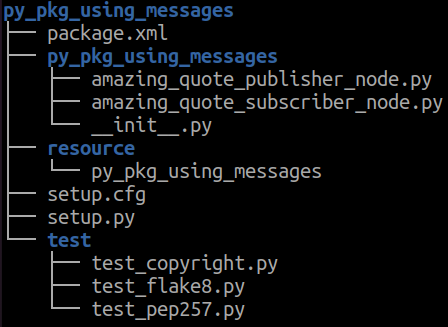
\includegraphics[width=\linewidth]{ros2_basics_figures/usual_package_form_with_nodes.png}
            \small \textit{Package with Publisher and Subscriber Nodes}
        \end{column}
        \begin{column}{0.33\textwidth}
            \centering
            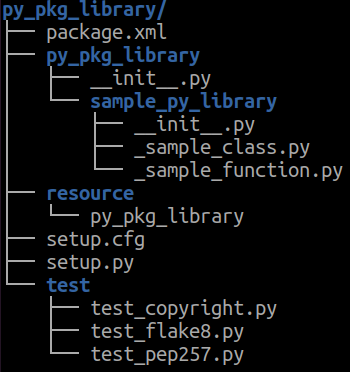
\includegraphics[width=\linewidth]{ros2_basics_figures/package_library.png}
            \small \textit{Library Package}
        \end{column}
        \begin{column}{0.33\textwidth}
            \centering
            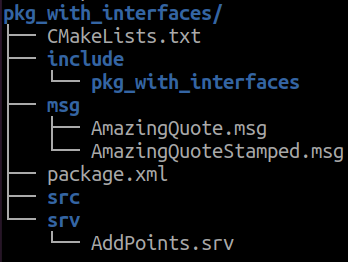
\includegraphics[width=\linewidth]{ros2_basics_figures/package_with_interfaces.png}
            \small \textit{Interfaces Package}
        \end{column}
    \end{columns}
    \bigskip
    Each Python package directory contains an inner folder that defines the main \textit{Python Module} (with the same name) where the source code is located, and some other build and packaging metadata, like \texttt{package.xml}, \texttt{setup.py} and \texttt{setup.cfg}. For the Interfaces Package, we are mainly interested in \texttt{msg} and \texttt{srv} (optionally \texttt{action}) folders, while the build metadata are \texttt{package.xml} and \texttt{CMakeLists.txt}.
\end{frame}

\subsection{Creating \& building a Package}
\begin{frame}{}
    \frametitle{\insertsection \ - \insertsubsection}
    \begin{columns}[c]
        \begin{column}{0.55\textwidth}
            \footnotesize
            We create a source folder \texttt{src/} in our \texttt{<ros2\_ws>} workspace and enter it:
            \begin{block}{}
                \scriptsize \texttt{mkdir \textasciitilde/<ros2\_ws>/src \&\& cd \textasciitilde/<ros2\_ws>/src}
            \end{block}
            To create a package (\texttt{ament\_cmake} for C++, instead of \texttt{ament\_python}):
            \begin{block}{}
                \scriptsize \texttt{ros2 pkg create <pkg\_name> --build-type ament\_python --dependencies rclpy <other\_pkg>}
            \end{block}
            We build from the \texttt{<ros2\_ws>} folder with \myhl{yellow}{\textbf{\texttt{colcon build}}}, which creates \texttt{build/}, \texttt{install/} and \texttt{log/}. After building, always type \myhl{yellow}{\textbf{\texttt{source install/setup.bash}}} to make the changes visible to your terminal.
            \medskip \\
            \texttt{ros2 pkg create -h} lists the creation options.
        \end{column}
        \begin{column}{0.45\textwidth}
            \centering
            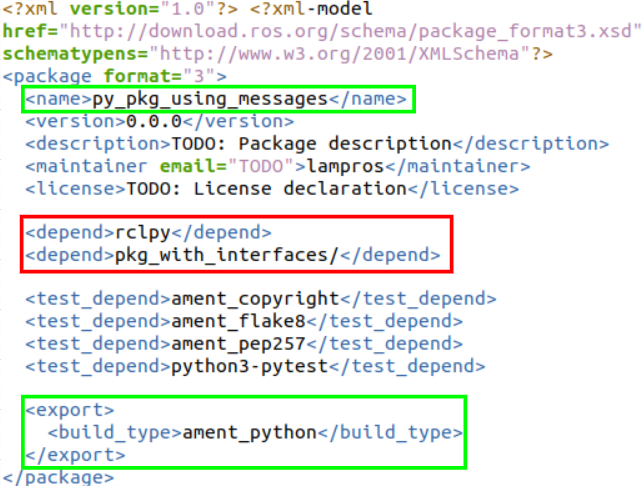
\includegraphics[width=\linewidth]{ros2_basics_figures/python_package_xml.png} \\
            \scriptsize \textit{\texttt{package.xml} of an \texttt{ament\_python} package; in red, lines you may need to add before building (mainly dependencies)}
        \end{column}
    \end{columns}
\end{frame}

\subsubsection{setup.py}
\begin{frame}{\insertsection \ - \insertsubsection \ - \insertsubsubsection}
    The \textbf{\texttt{setup.py}} file exists in \texttt{ament\_python} packages, but not in \texttt{ament\_cmake} ones (similarly with \texttt{setup.cfg} file).
    \vspace{0.5em}
    \begin{columns}[c]
        \begin{column}{0.6\textwidth}
            \centering
            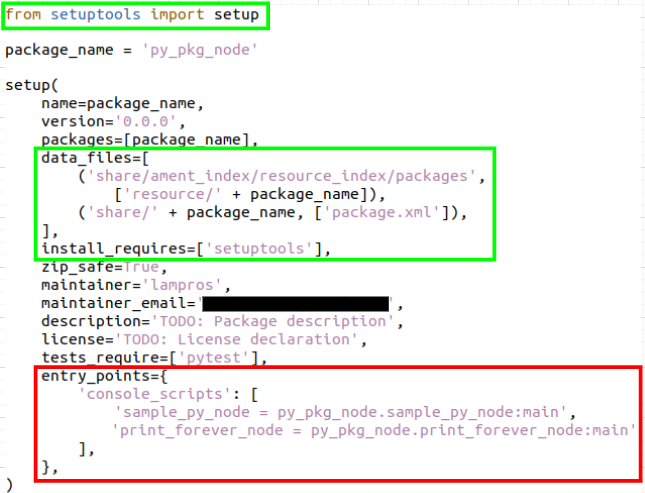
\includegraphics[width=\linewidth]{ros2_basics_figures/simple_python_setup_py.png} \\
            \small \textit{simple \texttt{setup.py} file}
        \end{column}
        \begin{column}{0.4\textwidth}
            \setbeamercolor{block title}{bg=red, fg=white}
            \setbeamercolor{block body}{bg=red!10, fg=black}
            \begin{block}{Important!}
                \small
                We should always add the executable nodes in the \texttt{console\_scripts} list (marked with red color).
            \end{block}
        \end{column}
    \end{columns}
\end{frame}

% Nodes
\section{Nodes}

\subsection{What is a Node?}
\begin{frame}{}
    \frametitle{\insertsection \ - \insertsubsection}
    \begin{columns}[c]
        \begin{column}{0.5\textwidth}
            \small
            \begin{enumerate}
                \item \textbf{Nodes} are \textbf{executable units} / processes, doing some computation.
                \item \textbf{Each device or algorithm} in our robotic system can be a \textbf{distinct node}.
                \item They are \textbf{decoupled} (no shared memory) but \textbf{talk to each other by using interfaces}, via \textbf{publish-subscribe} or \textbf{request-response}.
            \end{enumerate}
            \begin{block}{ROS2 Node Functionalities}
                \textbf{\texttt{ros2 node -h}}
            \end{block}
            \begin{block}{\textbf{create\_timer}}
                \scriptsize \texttt{\textbf{create\_timer}(timer\_period\_sec, callback)}
            \end{block}
        \end{column}
        \begin{column}{0.5\textwidth}
            \centering
            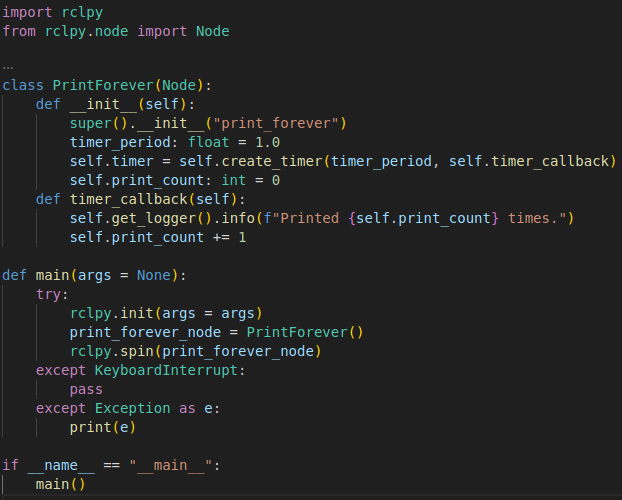
\includegraphics[width=\linewidth]{ros2_basics_figures/simple_ROS2_python_node.png} \\
            \small \textit{Simple ROS2 Python Node}
        \end{column}
    \end{columns}
\end{frame}

\begin{frame}{\insertsection \ - \insertsubsection}
    Let's assume that the node \texttt{print\_forever\_node.py} belongs to the package \texttt{py\_pkg\_node}. To make the node executable, we need to add it to the \texttt{console\_scripts} list in the \texttt{setup.py} file as it is shown right below (\texttt{<print\_forever\_node>} is chosen as the name of our node).
    \begin{block}{At the end of \texttt{setup.py} file}
        \small
        \texttt{entry\_points = \{'console\_scripts': ['print\_forever\_node = py\_pkg\_node.print\_forever\_node:main']\}}
    \end{block}
    \smallskip
    Now, after we build the modified package, we can type the command \ \texttt{ros2 run py\_pkg\_node print\_forever\_node} to run the node, or, in the general case:
    \begin{block}{Command to run a node}
        \large \textbf{\texttt{ros2 run <pkg\_name> <node\_name>}}
    \end{block}
    \smallskip
    To see the currently available (running) nodes, type \ \myhl{lightgray}{\textbf{\texttt{ros2 node list}}}.
\end{frame}


% ROS2 Communication System
\section{ROS2 Communication System}

\subsection{General Communication Scheme}
\begin{frame}{\insertsection \ - \insertsubsection}
    \begin{columns}[c]
        \begin{column}{0.2\textwidth}
            \small \textit{ROS2 General Communication Scheme}
        \end{column}
        \begin{column}{0.8\textwidth}
            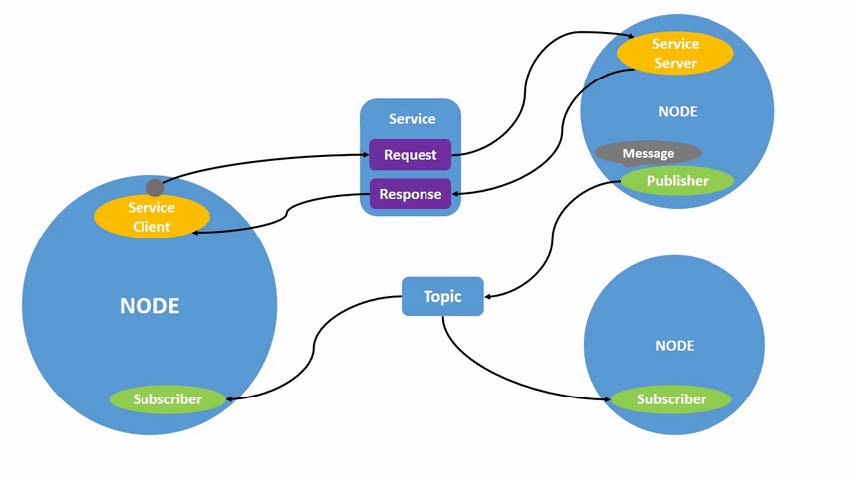
\includegraphics[width=\linewidth]{ros2_basics_figures/ros_communication_scheme.jpg}
        \end{column}
    \end{columns}
    \medskip
    Here we see a basic ROS 2 communication scheme consisting of three nodes. Each node can act as a \textbf{publisher}, \textbf{subscriber}, \textbf{service server}, or \textbf{service client}. They communicate using simple messages over topics, and request–response message pairs through services.
\end{frame}

\subsection{Interfaces}
\begin{frame}{\insertsection \ - \insertsubsection}
    Interfaces are files written in the ROS2 Interface Description Language (IDL). We can use them to communicate between nodes, that can even be written in different languages (Python, C++, ...). They are of 3 types:
    \begin{itemize}
        \item \textbf{Messages} $\rightarrow$ \texttt{.msg} files (simplest interface form)
        \item \textbf{Services} $\rightarrow$ \texttt{.srv} files (request \& response messages)
        \item \textbf{Actions} $\rightarrow$ \texttt{.action} files (mixture of messages and services)
    \end{itemize}
    Some very well-known interface packages are \textbf{\texttt{geometry\_msgs}} and \textbf{\texttt{sensor\_msgs}}. Of course, we can write our own interface packages.
    \begin{columns}[c]
        \begin{column}{0.45\textwidth}
            \begin{block}{ROS2 Interface Functionalities}
                \large \textbf{\texttt{ros2 interface -h}}
            \end{block}
        \end{column}
        \begin{column}{0.45\textwidth}
            \begin{block}{ros2 interface show geometry\_msgs/msg/Point}
                \small
                \texttt{\# This contains the position of a point in free space} \\
                \texttt{float64 x} \\
                \texttt{float64 y} \\
                \texttt{float64 z}
            \end{block}        
        \end{column}
    \end{columns}
\end{frame}

\subsubsection{Messages}
\begin{frame}{}
    \frametitle{\insertsection \ - \insertsubsection \ - \insertsubsubsection}
    \begin{columns}[c]
        \begin{column}{0.58\textwidth}
            \small
            \begin{enumerate}
                \item \textbf{Messages} (\texttt{.msg}) are data structures, the building blocks of communication over \textbf{topics}, \textbf{services}, and \textbf{actions}.
                \item A message consists of \textbf{typed fields} (e.g. \texttt{int32}, \texttt{float64}, \texttt{bool}, \texttt{string}, \texttt{time}).
                \item \textbf{Topics} are named communication channels (\textbf{buses}) that use \textbf{exclusively messages} as payload.
            \end{enumerate}
        \end{column}
        \begin{column}{0.42\textwidth}
            \begin{block}{ros2 interface show geometry\_msgs/msg/Pose}
                \scriptsize
                \texttt{\# A pose in free space, composed of position and orientation} \\
                \texttt{Point position} \\
                \texttt{Quaternion orientation}
            \end{block}
            \scriptsize \texttt{ros2 topic list}, \texttt{ros2 topic -h}
        \end{column}
    \end{columns}
    \centering
    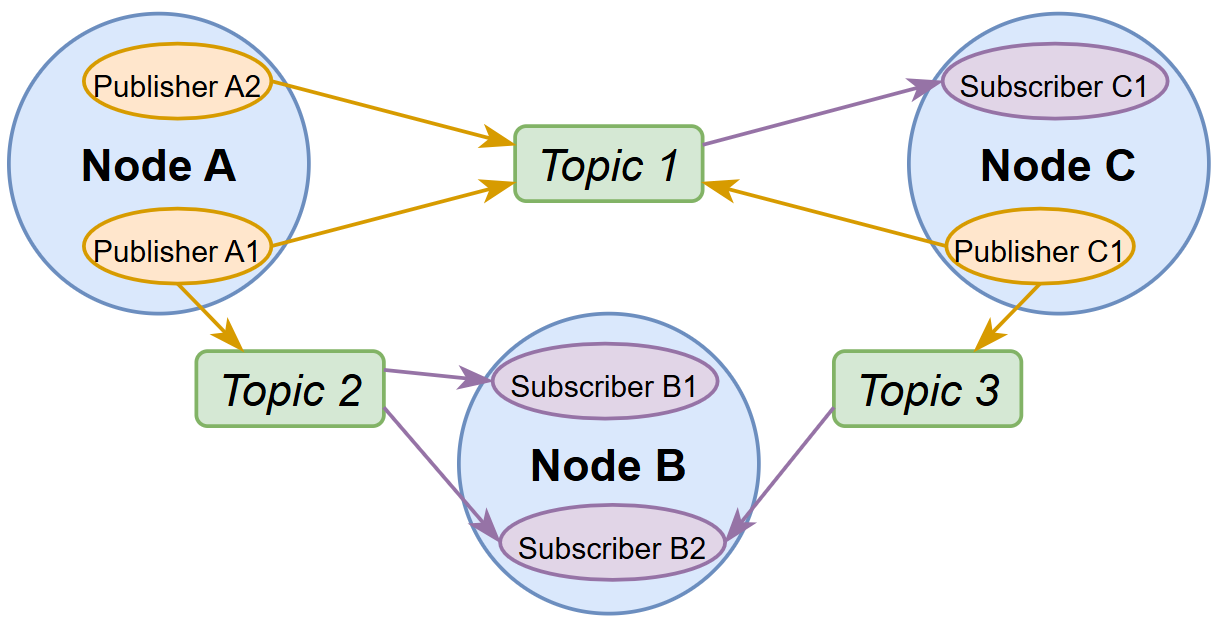
\includegraphics[height=0.42\textheight,keepaspectratio]{ros2_basics_figures/topics_publishers_subscribers.png} \\
    \scriptsize \textit{Topics, Publishers \& Subscribers: Example communication scheme}
\end{frame}

\subsubsection{Services}
\begin{frame}{}
    \frametitle{\insertsection \ - \insertsubsection \ - \insertsubsubsection}
    \small
    \begin{enumerate}
        \item A \textbf{Service} is similar to a topic, as both enable data exchange between nodes, but a topic is \textit{one-way} and \textit{continuous} (publish - subscribe), while a service is \textit{\textbf{two-way}} and \textit{\textbf{on-demand}} (request - response).
        \item Each service has a \textbf{\textit{single} Service Server}, that processes a \textbf{request} and sends back a \textbf{response}, and can have \textbf{\textit{multiple} Service Clients}.
    \end{enumerate}
    \begin{columns}[c]
        \begin{column}{0.42\textwidth}
            \begin{block}{\texttt{AddPoints.srv} (example)}
                \scriptsize
                \texttt{geometry\_msgs/Point a} \hfill \texttt{\# Req.} \\
                \texttt{geometry\_msgs/Point b} \\
                \texttt{---} \\
                \texttt{geometry\_msgs/Point result} \hfill \texttt{\# Resp.}
            \end{block}
        \end{column}
        \begin{column}{0.58\textwidth}
            \centering
            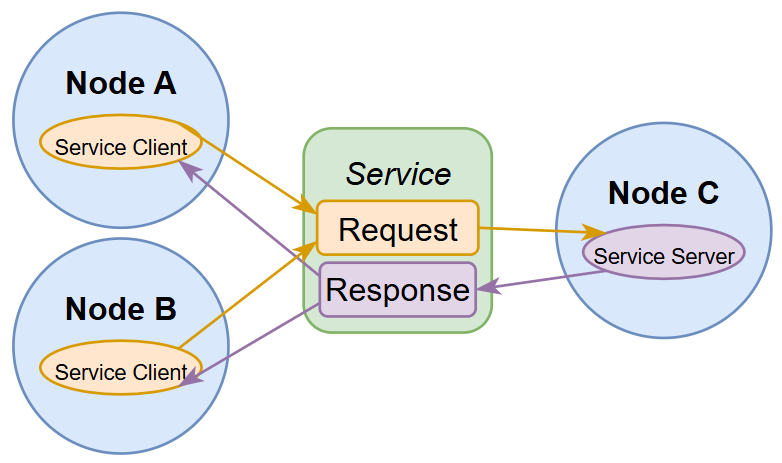
\includegraphics[height=0.4\textheight,keepaspectratio]{ros2_basics_figures/services_servers_clients.png} \\
            \scriptsize \textit{Services, Servers \& Clients: Example communication scheme}
        \end{column}
    \end{columns}
\end{frame}

\subsubsection{Actions}
\begin{frame}{\insertsection \ - \insertsubsection \ - \insertsubsubsection}
    \begin{enumerate}
        \item An \textbf{Action} is a \textbf{communication mechanism} similar to a service, as both provide \textit{two-way, on-demand} interaction.
        \item It differs from a service in the sense that it is designed for \textit{\textbf{long-running tasks}}, where the client may need
              \textbf{feedback} during execution, and the option to \textbf{cancel} the task.
        \item Each action is defined by three message structures:
              \begin{itemize}
                  \item \textbf{Goal} (sent by the client to the server)
                  \item \textbf{Result} (sent by the server after completion)
                  \item \textbf{Feedback} (sent by the server while executing)
              \end{itemize}
    \end{enumerate}
    \begin{block}{ros2 interface show nav2\_msgs/action/FollowWaypoints}
        \small
        \texttt{geometry\_msgs/PoseStamped[] poses} \hfill \texttt{\# Goal} \\
        \texttt{---} \\
        \texttt{int32[] missed\_waypoints} \hfill \texttt{\# Result} \\
        \texttt{---} \\
        \texttt{uint32 current\_waypoint} \hfill \texttt{\# Feedback} 
    \end{block}
\end{frame}

\subsection{Publisher \& Subscriber}
\begin{frame}{}
    \frametitle{\insertsection \ - \insertsubsection}
    \begin{columns}[t]
        \begin{column}{0.5\textwidth}
            \centering
            \begin{block}{\scriptsize \textbf{create\_publisher}}
                \scriptsize \texttt{(msg\_type, topic, qos\_profile)}
            \end{block}
            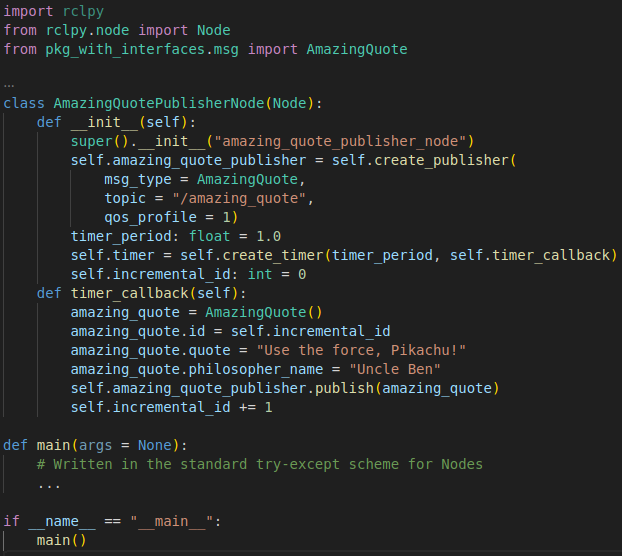
\includegraphics[height=0.42\textheight,keepaspectratio]{ros2_basics_figures/simple_ROS2_python_publisher.png} \\
            \scriptsize \textit{Simple ROS2 Python Publisher}
        \end{column}
        \begin{column}{0.5\textwidth}
            \centering
            \begin{block}{\scriptsize \textbf{create\_subscription}}
                \scriptsize \texttt{(msg\_type, topic, callback, qos\_profile)}
            \end{block}
            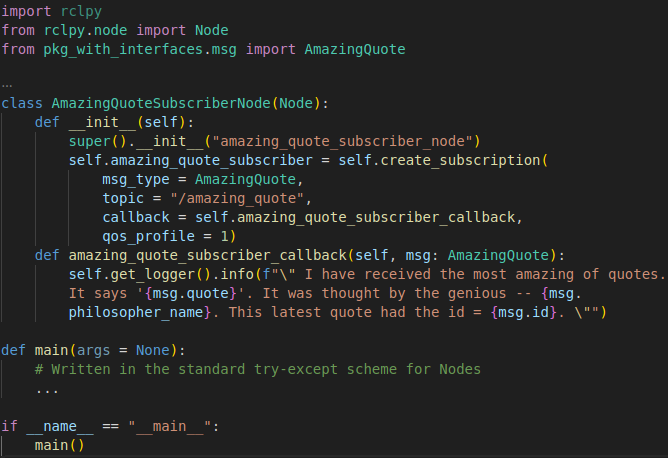
\includegraphics[height=0.42\textheight,keepaspectratio]{ros2_basics_figures/simple_ROS2_python_subscriber.png} \\
            \scriptsize \textit{Simple ROS2 Python Subscriber}
        \end{column}
    \end{columns}
    \setbeamercolor{block title}{bg=red, fg=white}
    \setbeamercolor{block body}{bg=red!10, fg=black}
    \begin{block}{\scriptsize Important!}
        \scriptsize A message from another package makes that package a dependency: add it to \texttt{package.xml}.
    \end{block}
\end{frame}

\subsection{Service Server \& Client}
\begin{frame}{}
    \frametitle{\insertsection \ - \insertsubsection}
    \begin{columns}[t]
        \begin{column}{0.5\textwidth}
            \centering
            \begin{block}{\scriptsize \textbf{create\_service}}
                \scriptsize \texttt{(srv\_type, srv\_name, callback)}
            \end{block}
            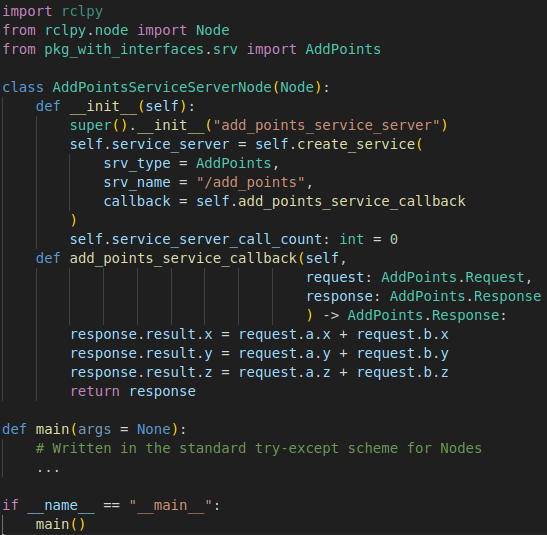
\includegraphics[height=0.62\textheight,keepaspectratio]{ros2_basics_figures/simple_ROS2_python_service_server.png} \\
            \scriptsize \textit{Simple ROS2 Python Service Server}
        \end{column}
        \begin{column}{0.5\textwidth}
            \centering
            \begin{block}{\scriptsize \textbf{create\_client}}
                \scriptsize \texttt{(srv\_type, srv\_name)}
            \end{block}
            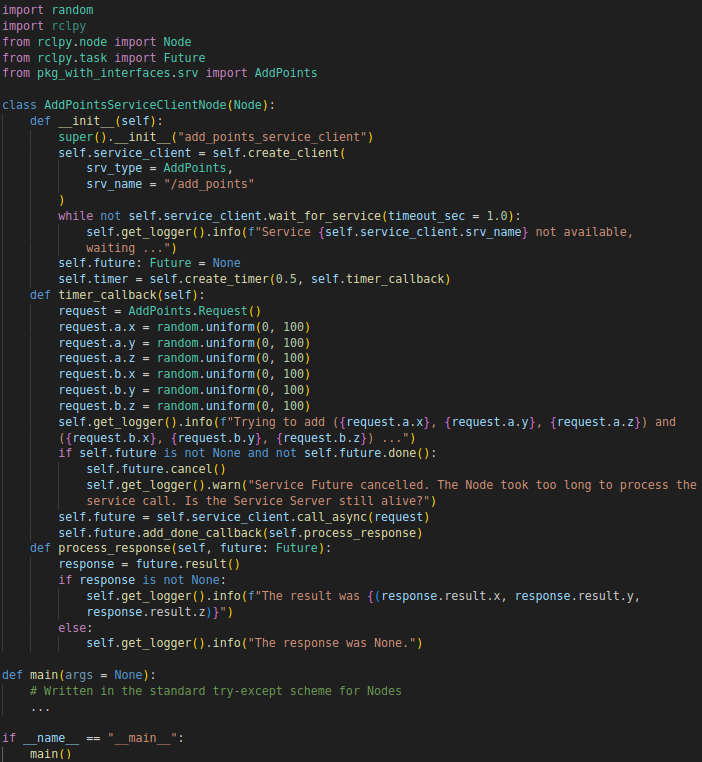
\includegraphics[height=0.62\textheight,keepaspectratio]{ros2_basics_figures/simple_ROS2_python_service_client.png} \\
            \scriptsize \textit{Simple ROS2 Python Service Client}
        \end{column}
    \end{columns}
\end{frame}


% Parameters
\section{Parameters}

\subsection{What are parameters?}
\begin{frame}{}
    \frametitle{\insertsection \ - \insertsubsection}
    \begin{columns}[c]
        \begin{column}{0.5\textwidth}
            \scriptsize
            \begin{enumerate}
                \item \textbf{Parameters} are key - value pairs owned by a node, making it more \textit{\textbf{reusable}} and \textit{\textbf{configurable}}: we \textbf{change its behavior} without modifying the source code (algorithm \textit{\textbf{tuning}}, \textit{\textbf{environment-specific configuration}}).
                \item They can be \textbf{static} (read once at startup) or \textbf{dynamic} (read periodically and updated at runtime via callbacks).
                \item They are set \textbf{programmatically} (rclpy, rclcpp), through \textbf{YAML files} or from the \textbf{CLI}.
            \end{enumerate}
            \begin{block}{}
                \scriptsize
                \textbf{\texttt{declare\_parameter(name, value)}} \\
                \textbf{\texttt{get\_parameter(name).value}}
            \end{block}
        \end{column}
        \begin{column}{0.5\textwidth}
            \centering
            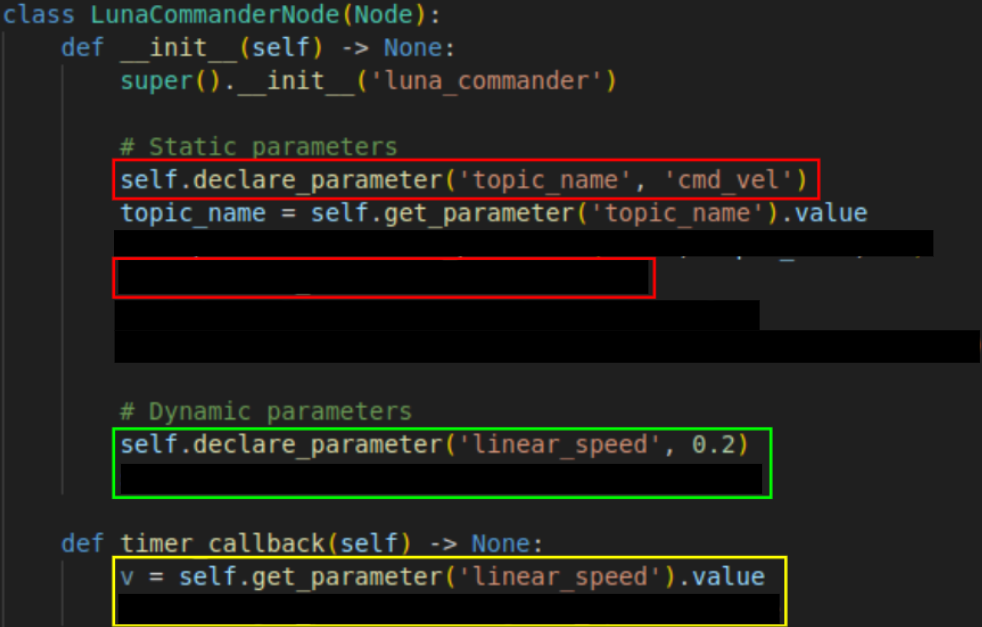
\includegraphics[width=\linewidth]{ros2_basics_figures/declare_parameters_luna.png} \\
            \scriptsize \textit{parameters declared for the \texttt{luna\_commander} node}
            \vspace{3pt} \\
            \raggedright \scriptsize
            \myhl{Peach}{\textit{static}}: \myhl{red}{\texttt{period}}, \myhl{red}{\texttt{topic\_name}}. \myhl{LimeGreen}{\textit{dynamic}}: \myhl{green}{\texttt{linear\_speed}}, \myhl{green}{\texttt{angular\_speed}} (read in the \texttt{timer\_callback}). \texttt{period} could be dynamic with \texttt{add\_on\_set\_parameters\_callback} (next slide).
        \end{column}
    \end{columns}
\end{frame}

\subsection{Manage parameters}
\begin{frame}{}
    \frametitle{\insertsection \ - \insertsubsection}
    \begin{columns}[t]
        \begin{column}{0.5\textwidth}
            \scriptsize
            \textbf{CLI} (while the node runs): \myhl{lightgray}{\texttt{ros2 param list}}; \texttt{get} works on static \& dynamic parameters, \texttt{set} only on dynamic ones.
            \begin{block}{}
                \texttt{ros2 param get /<node> <param>} \\
                \texttt{ros2 param set /<node> <param> <value>} \\
                \texttt{ros2 param dump /<node> --output-dir <dir>} \\
                \texttt{ros2 param load /<node> <file>}
            \end{block}
            \textbf{Reacting to changes} (\textbf{validate} values, \textbf{adjust timers}, \textbf{log}): register \myhl{lightgray}{\texttt{add\_on\_set\_parameters\_callback}}; it gets the parameters (\texttt{name}, \texttt{type\_}, \texttt{value}) and returns a \textbf{\texttt{SetParametersResult}} to accept or reject the change.
        \end{column}
        \begin{column}{0.5\textwidth}
            \scriptsize
            \textbf{YAML files} store and reload the parameters of a node (good practice: a \myhl{yellow}{\texttt{config} folder} in the package):
            \begin{itemize}
                \item top-level key: the \texttt{<node\_name>}
                \item parameters under the key \texttt{ros\_\_parameters}
                \item \textit{integers}, \textit{floats}, \textit{strings}, \textit{booleans}, \textit{lists}, ...
            \end{itemize}
            \centering
            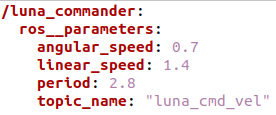
\includegraphics[width=0.7\linewidth]{ros2_basics_figures/YAML_file_example.png}
        \end{column}
    \end{columns}
    \vspace{4pt}
    \centering
    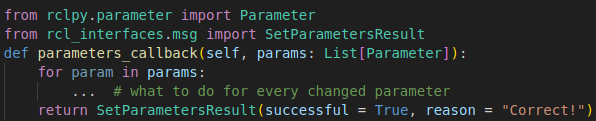
\includegraphics[width=0.9\linewidth]{ros2_basics_figures/add_on_set_parameters_callback_example.png}
\end{frame}

% Launch files
\section{Launch files}

\subsection{What are launch files?}
\begin{frame}{}
    \frametitle{\insertsection \ - \insertsubsection}
    \begin{columns}[c]
        \begin{column}{0.5\textwidth}
            \footnotesize
            \begin{enumerate}
                \item A \textbf{launch file} is a \textit{\textbf{Python script}} that \textit{\textbf{starts}} and \textit{\textbf{configures}} multiple \textbf{ROS2 nodes} together (written in any language).
                \item It provides \textbf{automation} (several nodes, one command), \textbf{configuration} (parameters, remappings, arguments) and \textbf{reusability} across experiments.
                \item Good practice: save them in a \myhl{yellow}{\texttt{launch} folder} of the package.
            \end{enumerate}
            \begin{block}{ROS2 Launch Functionalities}
                \textbf{\texttt{ros2 launch -h}}
            \end{block}
        \end{column}
        \begin{column}{0.5\textwidth}
            \centering
            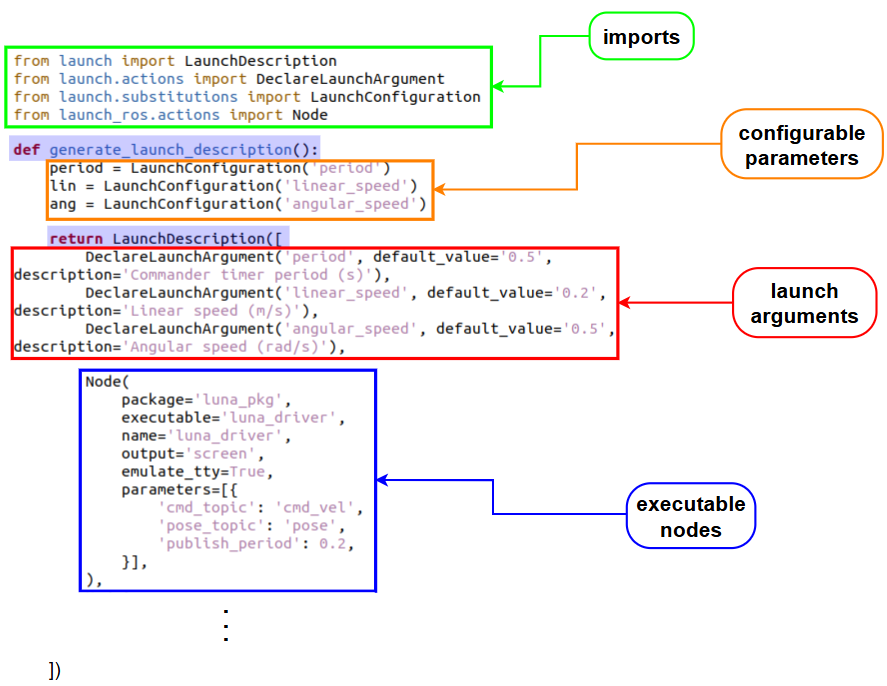
\includegraphics[width=\linewidth]{ros2_basics_figures/launch_file_example.png} \\
            \scriptsize \textit{launch file simple example}
        \end{column}
    \end{columns}
\end{frame}

\subsection{Running a launch file}
\begin{frame}{}
    \frametitle{\insertsection \ - \insertsubsection}
    \begin{enumerate}
        \item To execute a launch file we use:
              \begin{block}{\textbf{Run a launch file}}
                  \large \textbf{\texttt{ros2 launch <package\_name> <launch\_file\_name> <launch\_arguments>}}
              \end{block}
        \item This will start all the nodes defined in the file, with the specified parameters and remappings.
    \end{enumerate}
    \vspace{1em}
    \centering
    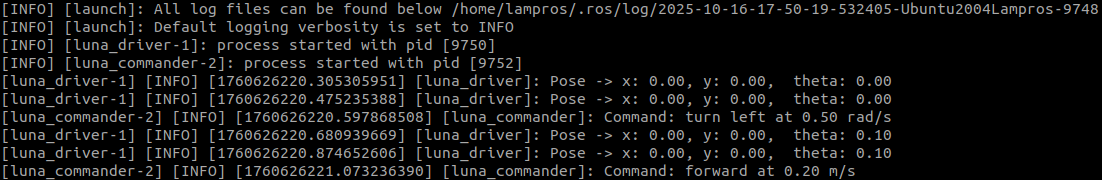
\includegraphics[width=\linewidth]{ros2_basics_figures/ros2_run_launch_file_example.png}
    \footnotesize \textit{Here we launch the nodes /luna\_driver and /luna\_commander with:} \\ \texttt{ros2 launch luna\_package luna\_package\_launch.py} \\
    \vspace{5pt}
    \footnotesize \textit{We could also launch like this to change some parameters:} \\ \texttt{ros2 launch luna\_package luna\_package\_launch.py period:=2.0 linear\_speed:=10.0 angular\_speed:=1.0}
\end{frame}


% Managing ROS2 Graph activity
\section{Inspecting ROS2 Graph activity}

\subsection{Parameters}
\begin{frame}{}
    \frametitle{\insertsection \ - \insertsubsection}
    \begin{block}{Output a list of available parameters}
        \begin{columns}[c]
            \begin{column}{0.5\textwidth}
                \centering
                \large \textbf{\texttt{ros2 param list}}
            \end{column}
            \begin{column}{0.5\textwidth}
                \centering
                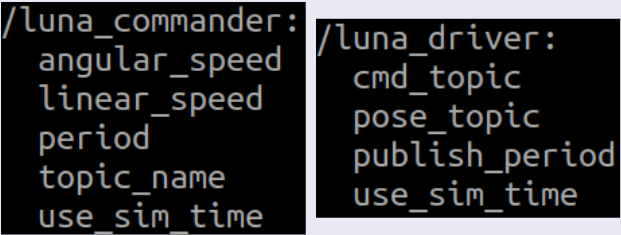
\includegraphics[width=0.7\linewidth]{ros2_basics_figures/ros2_param_list_example.png}
            \end{column}
        \end{columns}
    \end{block}
    \begin{block}{Get parameter}
        \begin{columns}[c]
            \begin{column}{0.5\textwidth}
                \centering
                \large \textbf{\texttt{ros2 param get /<node\_name> <parameter\_name>}}
            \end{column}
            \begin{column}{0.5\textwidth}
                \centering
                \small \texttt{ros2 param get /luna\_driver publish\_period}
                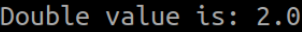
\includegraphics[width=0.6\linewidth]{ros2_basics_figures/ros2_param_get_example.png}
            \end{column}
        \end{columns}
    \end{block}
    \begin{block}{Set parameter}
        \begin{columns}[c]
            \begin{column}{0.5\textwidth}
                \centering
                \large \textbf{\texttt{ros2 param set /<node\_name> <parameter\_name> <value>}}
            \end{column}
            \begin{column}{0.5\textwidth}
                \centering
                \small \texttt{ros2 param set /luna\_commander linear\_speed 0.7}
                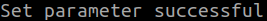
\includegraphics[width=0.7\linewidth]{ros2_basics_figures/ros2_param_set_example.png}
            \end{column}
        \end{columns}
    \end{block}
    \vspace{5pt}
\end{frame}

\begin{frame}{}
    \frametitle{\insertsection \ - \insertsubsection}
    \begin{block}{Dump the parameters of a node to a yaml file}
        \begin{columns}[c]
            \begin{column}{0.5\textwidth}
                \centering
                \large \textbf{\texttt{ros2 param dump /<node\_name>}}
            \end{column}
            \begin{column}{0.5\textwidth}
                \centering
                \small \texttt{ros2 param dump /luna\_commander --output-dir config/}
                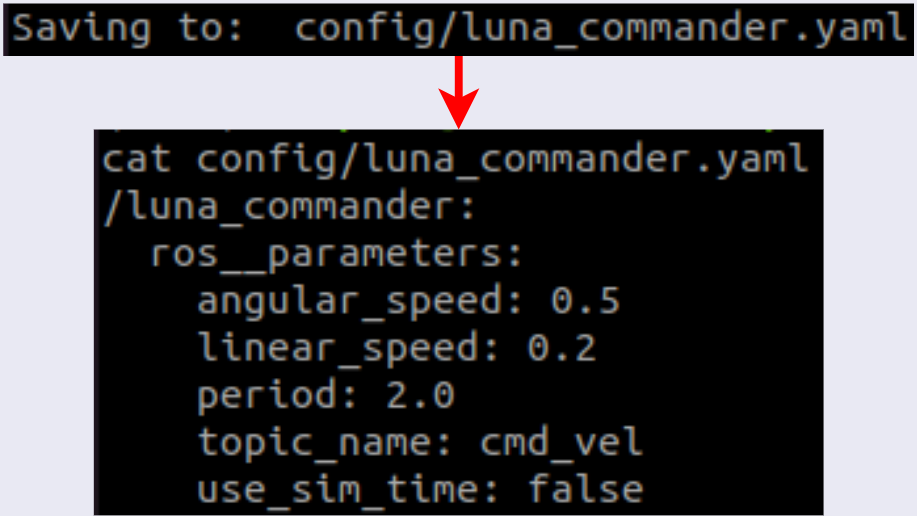
\includegraphics[width=0.8\linewidth]{ros2_basics_figures/ros2_param_dump_example.png}
            \end{column}
        \end{columns}
    \end{block}
    \begin{block}{Load parameter file for a node}
        \begin{columns}[c]
            \begin{column}{0.5\textwidth}
                \centering
                \large \textbf{\texttt{ros2 param load /<node\_name> <parameter\_file>}}
            \end{column}
            \begin{column}{0.5\textwidth}
                \centering
                \small \texttt{ros2 param load /luna\_commander config/luna\_commander.yaml}
                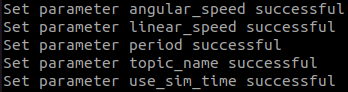
\includegraphics[width=0.7\linewidth]{ros2_basics_figures/ros2_param_load_example.png}
            \end{column}
        \end{columns}
    \end{block}
\end{frame}

\subsection{Nodes}
\begin{frame}{}
    \frametitle{\insertsection \ - \insertsubsection}
    \begin{block}{Output a list of available nodes}
        \begin{columns}[c]
            \begin{column}{0.4\textwidth}
                \centering
                \large \textbf{\texttt{ros2 node list}}
            \end{column}
            \begin{column}{0.6\textwidth}
                \centering
                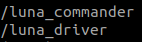
\includegraphics[width=0.6\linewidth]{ros2_basics_figures/ros2_node_list_example.png}
            \end{column}
        \end{columns}
    \end{block}
    \begin{block}{Output information about a node}
        \begin{columns}[c]
            \begin{column}{0.4\textwidth}
                \centering
                \large \textbf{\texttt{ros2 node info /<node\_name>}}
            \end{column}
            \begin{column}{0.6\textwidth}
                \centering
                \small \texttt{ros2 node info /luna\_driver} \\
                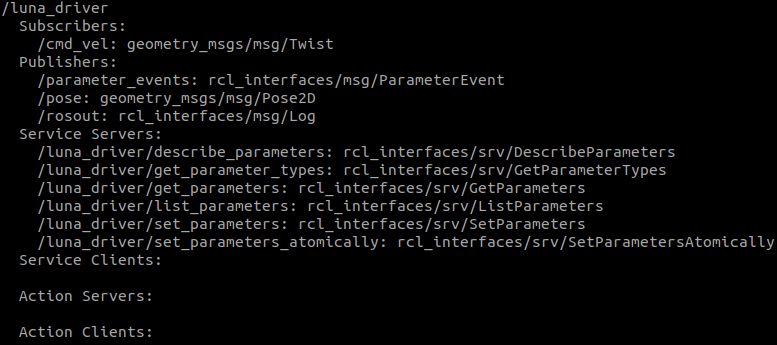
\includegraphics[width=1.0\linewidth]{ros2_basics_figures/ros2_node_info_example.png}
            \end{column}
        \end{columns}
    \end{block}
\end{frame}

\subsection{Topics}
\begin{frame}{}
    \frametitle{\insertsection \ - \insertsubsection}
    \begin{block}{Output a list of available topics}
        \begin{columns}[c]
            \begin{column}{0.5\textwidth}
                \centering
                \large \textbf{\texttt{ros2 topic list}}
            \end{column}
            \begin{column}{0.5\textwidth}
                \centering
                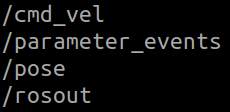
\includegraphics[width=0.4\linewidth]{ros2_basics_figures/ros2_topic_list_example.png}
            \end{column}
        \end{columns}
    \end{block}
    \begin{block}{Output information about a topic}
        \begin{columns}[c]
            \begin{column}{0.5\textwidth}
                \centering
                \large \textbf{\texttt{ros2 topic info /<topic\_name>}}
            \end{column}
            \begin{column}{0.5\textwidth}
                \centering
                \small \texttt{ros2 topic info /pose} \\
                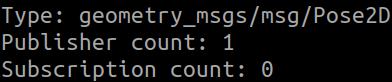
\includegraphics[width=0.8\linewidth]{ros2_basics_figures/ros2_topic_info_example.png}
            \end{column}
        \end{columns}
    \end{block}
    \begin{block}{Output messages from a topic}
        \begin{columns}[c]
            \begin{column}{0.5\textwidth}
                \centering
                \large \textbf{\texttt{ros2 topic echo /<topic\_name>}}
            \end{column}
            \begin{column}{0.5\textwidth}
                \centering
                \small \texttt{ros2 topic echo /pose} \\
                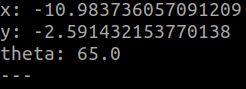
\includegraphics[width=0.6\linewidth]{ros2_basics_figures/ros2_topic_echo_example.png}
            \end{column}
        \end{columns}
    \end{block}
\end{frame}

\begin{frame}{}
    \frametitle{\insertsection \ - \insertsubsection}
    \begin{block}{Publish a message to a topic}
        \centering
        \small \textbf{\texttt{ros2 topic pub -r <Hz> /<topic\_name> <message\_type> <values>}}
        \vspace{5pt} \\
        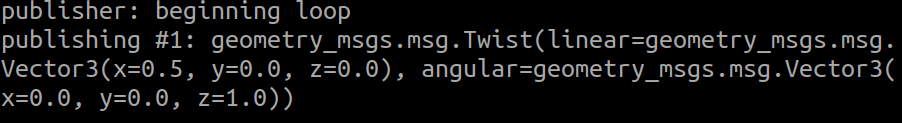
\includegraphics[width=0.7\linewidth]{ros2_basics_figures/ros2_topic_pub_example.png} \\
        \small \texttt{ros2 topic pub -r 2 /cmd\_vel geometry\_msgs/msg/Twist "{linear: {x: 0.5, y: 0.0, z: 0.0}, angular: {x: 0.0, y: 0.0, z: 1.0}}"}
    \end{block}
    \begin{block}{Print a topic's type}
        \begin{columns}[c]
            \begin{column}{0.5\textwidth}
                \centering
                \normalsize \textbf{\texttt{ros2 topic type /<topic\_name>}}
            \end{column}
            \begin{column}{0.5\textwidth}
                \centering
                \small \texttt{ros2 topic type /cmd\_vel} \\
                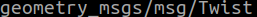
\includegraphics[width=0.7\linewidth]{ros2_basics_figures/ros2_topic_type_example.png}
            \end{column}
        \end{columns}
    \end{block}
    \begin{block}{Output a list of available topics of a given type}
        \begin{columns}[c]
            \begin{column}{0.5\textwidth}
                \centering
                \normalsize \textbf{\texttt{ros2 topic find <topic\_type>}}
            \end{column}
            \begin{column}{0.5\textwidth}
                \centering
                \small \texttt{ros2 topic find geometry\_msgs/msg/Twist} \\
                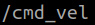
\includegraphics[width=0.2\linewidth]{ros2_basics_figures/ros2_topic_find_example.png}
            \end{column}
        \end{columns}
    \end{block}
\end{frame}

\subsection{Services}
\begin{frame}{}
    \frametitle{\insertsection \ - \insertsubsection}
    \begin{block}{Output a list of available services}
        \centering
        \normalsize \textbf{\texttt{ros2 service list}} \\
        \small \texttt{/luna\_commander/get\_parameters}, \texttt{/luna\_commander/set\_parameters}, \texttt{/luna\_commander/list\_parameters}, ...
    \end{block}
    \begin{block}{Output a service's type}
        \centering
        \normalsize \textbf{\texttt{ros2 service type /<service\_name>}} \\
        \footnotesize \texttt{ros2 service type /luna\_commander/get\_parameters} $\rightarrow$ \texttt{rcl\_interfaces/srv/GetParameters}
    \end{block}
    \begin{block}{Output a list of available services of a given type}
        \centering
        \normalsize \textbf{\texttt{ros2 service find <service\_type>}} \\
        \small \texttt{ros2 service find rcl\_interfaces/srv/GetParameters}
    \end{block}
    \begin{block}{Show the request \& response structure of a service type}
        \centering
        \normalsize \textbf{\texttt{ros2 interface show <service\_type>}} \\
        \small \texttt{ros2 interface show rcl\_interfaces/srv/GetParameters}
    \end{block}
\end{frame}

\begin{frame}[fragile]{\insertsection \ - \insertsubsection}
    \begin{block}{Call a service}
        \centering
        \normalsize \textbf{\texttt{ros2 service call /<service\_name> <service\_type> <values>}}
    \end{block}
    \begin{lstlisting}
ros2 service call /luna_commander/get_parameters rcl_interfaces/srv/GetParameters "{names: ['linear_speed']}"
    \end{lstlisting}
    \bigskip
    \begin{enumerate}
        \item The command above is, in essence, what \texttt{ros2 param get /luna\_commander linear\_speed} does behind the scenes: the \textbf{parameters} of a node are served through \textbf{services}!
        \item With the option \texttt{-r <Hz>} the call is repeated periodically.
    \end{enumerate}
\end{frame}

% Luna the Rover Exercise
\section{Luna the Rover Exercise}
\begin{frame}{}
    \frametitle{\insertsection}
    \begin{tikzpicture}[remember picture,overlay]
        \node[opacity=0.40, at=(current page.center)] {
            
\includegraphics[width=\paperwidth,height=\paperheight]{ros2_basics_figures/Luna_the_Rover.png}
        };
    \end{tikzpicture}
    {\centering
    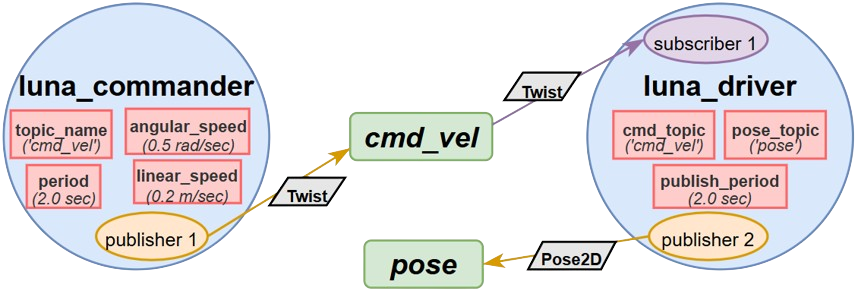
\includegraphics[width=\textwidth]{ros2_basics_figures/luna_robot_graph.png}}
    \\
    \vspace{1em}
    We are going to simulate a robot called \textit{\textbf{Luna}}, moving in 2D space. The \textbf{\texttt{luna\_commander}} node randomly generates velocity commands and publishes them as \textit{\texttt{Twist}} messages. The \textbf{\texttt{luna\_driver}} node subscribes to these commands, integrates them over time, and updates the robot’s 2D pose, publishing it continuously as \textit{\texttt{Pose2D}} messages. We can see that each node owns some key-value pairs, which we call \textbf{parameters} (see the Parameters section).
\end{frame}

% LED Exercise
\section{LED Exercise}
\begin{frame}{}
    \frametitle{\insertsection}
    \begin{columns}[c]
        \begin{column}{0.5\textwidth}
            \centering
            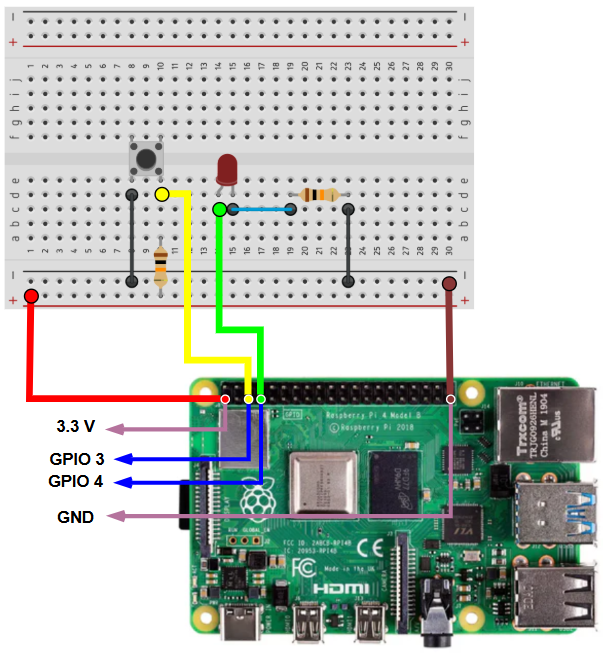
\includegraphics[width=\linewidth]{ros2_basics_figures/RPi_LED_circuit2.png}
            \small \textit{RPi4 - LED circuit scheme}
        \end{column}
        \begin{column}{0.5\textwidth}
            Let's test our ROS2 skills! Our goal: control a simple LED. We need:
            \begin{itemize}
                \item 1 RPi4
                \item 1 breadboard
                \item 1 LED
                \item 2 resistors (e.g. $10\,\text{k}\Omega$)
                \item 1 Button
                \item connecting wires
            \end{itemize}
            \setbeamercolor{block title}{bg=red, fg=white}
            \setbeamercolor{block body}{bg=red!10, fg=black}
            \begin{block}{\textbf{Important!}}
                \small
                Be very careful \textbf{not to short the 3.3V and GND pins!} At best, this might cause the RPi4 to reboot, but in the worst case, it could damage the board!
            \end{block}
        \end{column}
    \end{columns}
\end{frame}

\subsection{Custom Interface: LedValue}
\begin{frame}[fragile]{\insertsection \ - \insertsubsection}
    \begin{columns}[c]
        \begin{column}{0.5\textwidth}
            For the LED we define \textbf{our own message}, inside a separate \textbf{interfaces package} (\texttt{ament\_cmake}, see the \emph{Interfaces Package} structure from before):
            \begin{lstlisting}
leds_rpi_pkg_interfaces/
  msg/LedValue.msg
  CMakeLists.txt
  package.xml
            \end{lstlisting}
            Our nodes depend on it, so \texttt{leds\_rpi\_pkg} lists \texttt{leds\_rpi\_pkg\_interfaces} as a dependency in its \texttt{package.xml}.
        \end{column}
        \begin{column}{0.5\textwidth}
            \begin{block}{\texttt{msg/LedValue.msg}}
                \small
                \texttt{\# 0 $\rightarrow$ LED is OFF} \\
                \texttt{\# 1 $\rightarrow$ LED is ON} \\
                \texttt{uint32 led\_value}
            \end{block}
            \begin{block}{Check it after building}
                \scriptsize \texttt{ros2 interface show \\ leds\_rpi\_pkg\_interfaces/msg/LedValue}
            \end{block}
            \setbeamercolor{block title}{bg=red, fg=white}
            \setbeamercolor{block body}{bg=red!10, fg=black}
            \begin{block}{Important!}
                \small
                Build and source the workspace \textbf{before} using the new message in a node.
            \end{block}
        \end{column}
    \end{columns}
\end{frame}

\subsection{Tasks}
\begin{frame}{}
    \frametitle{\insertsection \ - \insertsubsection}
    \begin{columns}[t]
        \begin{column}{0.58\textwidth}
            \footnotesize
            \begin{enumerate}
                \item \textbf{Blink LED:} a \textit{publisher node} sends \textbf{alternating 0 and 1} (our \texttt{LedValue} message) every 1 second over a topic. A \textit{subscriber node} listens to it and its \textbf{callback blinks the LED}.
                \item \textbf{Change blink rate:} \textbf{declare a parameter} for the timer's period and update the timer when it changes (it is only created at startup!). Try it on the circuit: \\ \texttt{\scriptsize ros2 param set /blink\_led\_publisher blink\_led\_period 0.5}
                \item \textbf{Add button:} a \textit{second publisher node} reads a push button (pull-up resistor): LED \textbf{ON} while \textbf{pressed}, \textbf{OFF} when \textbf{released}. It publishes on the same topic, to the same subscriber.
                \item \textbf{Launch files:} one for the blinking LED and one for the button, each starting its publisher together with the LED subscriber.
            \end{enumerate}
        \end{column}
        \begin{column}{0.42\textwidth}
            \begin{block}{\small RPi.GPIO commands}
                \scriptsize
                \myhl{pink}{\texttt{RPi.GPIO.setmode(RPi.GPIO.BCM)}} \\
                \myhl{pink}{\texttt{RPi.GPIO.setup(pin, RPi.GPIO.OUT)}} \\
                \myhl{pink}{\texttt{RPi.GPIO.input(pin)}} \hfill reads 0/1 \\
                \myhl{pink}{\texttt{RPi.GPIO.output(pin, value)}}
            \end{block}
            \centering
            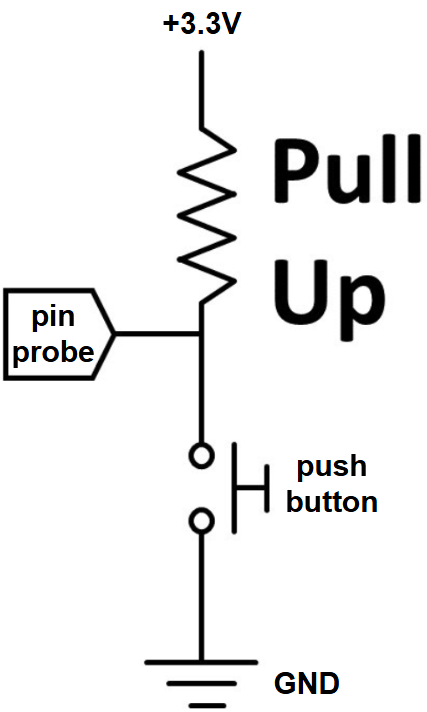
\includegraphics[width=0.5\linewidth]{ros2_basics_figures/pullup_resistor_configuration.png} \\
            \tiny \href{https://www.youtube.com/watch?v=aPVMKyZpaPA}{\textit{Push button with pull-up resistor}}: released $\rightarrow$ pin HIGH via the resistor, pressed $\rightarrow$ pin connected to GND, reads LOW.
        \end{column}
    \end{columns}
\end{frame}

% References
\section{References}
\begin{frame}{}
    \frametitle{\insertsection}
    \begin{itemize}
        \item \href{https://www.ros.org/}{\textbf{ROS Home}}
        \item \href{https://docs.ros.org/en/foxy/index.html}{\textbf{ROS2 Documentation for all distros, here for Foxy}}
        \item \href{https://docs.ros.org/en/iron/p/rclpy/rclpy.html}{\textbf{rclpy library documentation}}
        \item \href{https://ros2-tutorial.readthedocs.io/\_/downloads/en/latest/pdf/}{\textbf{Murilo's ROS2 Tutorial}}
        \item \href{https://www.youtube.com/watch?v=sWw69pIiMz0&list=PLSK7NtBWwmpTS_YVfjeN3ZzIxItI1P_Sr&index=5}{\textbf{Kevin Wood ROS2 Youtube Tutorials}}
        \item \href{https://docs.ros.org/en/foxy/Tutorials/Beginner-CLI-Tools/Understanding-ROS2-Parameters/Understanding-ROS2-Parameters.html}{\textbf{Understanding Parameters in ROS2}}
        \item \href{https://roboticsbackend.com/ros2-yaml-params/}{\textbf{ROS2 YAML files for parameters}}
        \item \href{https://www.theengineeringprojects.com/2021/03/what-is-raspberry-pi-4-pinout-specs-projects-datasheet.html}{\textbf{Raspberry Pi 4 introduction and basics}}
        \item \textbf{Control LED with RPi4 \& ROS2:} \href{https://medium.com/@alfredgithinji87/blinking-led-with-ros2-microros-and-an-esp32-c5b2cc6bcb12}{\textbf{here\_1}} \textbf{\&} \href{https://medium.com/nerd-for-tech/blink-led-with-raspberry-pi-foolproof-7f2584fd552a}{\textbf{here\_2}}
        \item \href{https://docs.elephantrobotics.com/docs/myarm-pi-300-en/2-serialproduct/2.12-myArm/2.12-myArm.html}{\textbf{Elephant Robotics Documentation}}
    \end{itemize}
\end{frame}


\end{document}
